
\documentclass{package/notes}
\usepackage[english]{babel}
\usepackage{amssymb,amsmath,amsfonts}  %%% for maths
%%%%%%%%%%%%%%%%%%%%%%%%%%%%%%%%%%%%%
\usepackage{package/color-env}
\usepackage{graphicx}
\usepackage{lipsum}
\renewcommand\qedsymbol{$\blacksquare$}
%%%%%%%%%%%%%%%%%%%%%%%%%%%%%%%%%%%%%

\begin{document}

	\begin{titlepage} % Suppresses headers and footers on the title page
		
		\centering % Centre everything on the title page
		
		\scshape % Use small caps for all text on the title page
		
		\vspace*{\baselineskip} % White space at the top of the page
		
		%------------------------------------------------
		%	Title
		%------------------------------------------------
		
		\rule{\textwidth}{1.6pt}\vspace*{-\baselineskip}\vspace*{2pt} % Thick horizontal rule
		\rule{\textwidth}{0.4pt} % Thin horizontal rule
		
		\vspace{0.75\baselineskip} % Whitespace above the title
		
		{\huge TITLE\\} % Title
		
		\vspace{0.75\baselineskip} % Whitespace below the title
		
		\rule{\textwidth}{0.4pt}\vspace*{-\baselineskip}\vspace{3.2pt} % Thin horizontal rule
		\rule{\textwidth}{1.6pt} % Thick horizontal rule
		
		\vspace{2\baselineskip} % Whitespace after the title block
		
		%------------------------------------------------
		%	Subtitle
		%------------------------------------------------
		
		\LARGE{AP CALCULUS NOTES} 
		
		\vspace*{3\baselineskip} % Whitespace under the subtitle
		
		
		
		\vspace{0.5\baselineskip} 
		
		
		
		\vspace{0.5\baselineskip} 
		
		
		
		\vfill 
		
		%------------------------------------------------
		% Author
		%------------------------------------------------
		
		
		\vspace{0.3\baselineskip} 
		
		
		{\large Edited by\\  Trevor Bushnell } 
		
	\end{titlepage}
	\tableofcontents
%\newpage
\chapter{Limits and Continuity}

\section{Introducing Calculus: Can Change Occur at an Instant?}
\begin{itemize}
	\item Traditional algebra uses relationships such as $\frac{\Delta y}{\Delta x}$ to model relationships
	\begin{itemize}
		\item However, this model falls apart because if $\Delta y = 0$ and $\Delta x = 0$, then the result is $\frac{0}{0}$ which is indeterminant
		\begin{itemize}
			\item \textbf{indeterminant} means that there might be a possible solution, but we cannot determine what that possible solution could be based on the current problem solving method
		\end{itemize}
	\end{itemize}

	\item We can use the \textbf{limit} to allow us to define change that occurs instantaneously in terms of incredibly small average rates in change (for example, doing $\Delta x = 0.000001$ instead of $\Delta x = 1$ or $\Delta x = 0.5$)
	\item Calculus uses limits to understand and model more precise/instantaneous change that algebra cannot answer
\end{itemize}

\section{Defining Limits and Using Limit Notation}
\begin{definition}
	GGiven a function $f$, the limit of $f(x)$ as $x$ approaches $c$ is a real number $R$ if $f(x)$ can be made arbitrarily close to $R$ by taking $x$ extremely close to $c$ (but \textit{not equal to} $c$).
	\newline\newline
	If the limit exists and is a real number, then:
	$$ \lim_{x\to c}f(x) = R$$
\end{definition}

\begin{itemize}
	\item A limit can be expressed graphically, numerically, or analytically
\end{itemize}
\newpage

\section{Estimating Limits From Graphs}

\begin{itemize}
	\item ONE SIDED LIMIT: A limit where you approach from a specific direction (either the left or the right)
	\begin{itemize}
		\item LHL (Left Hand Limit): $\lim_{x\to c^-} f(x) = L$
		\item RHL (Right Hand Limit): $\lim_{x\to c^+} f(x) = L$
		\item A limit exists if the left hand limit equals the right hand limit (LHL = RHL)
	\end{itemize}
	\item Using the information provided on a graph can help you interpret the limit of a function
\end{itemize}

\begin{figure*}[h]
	\begin{center}
		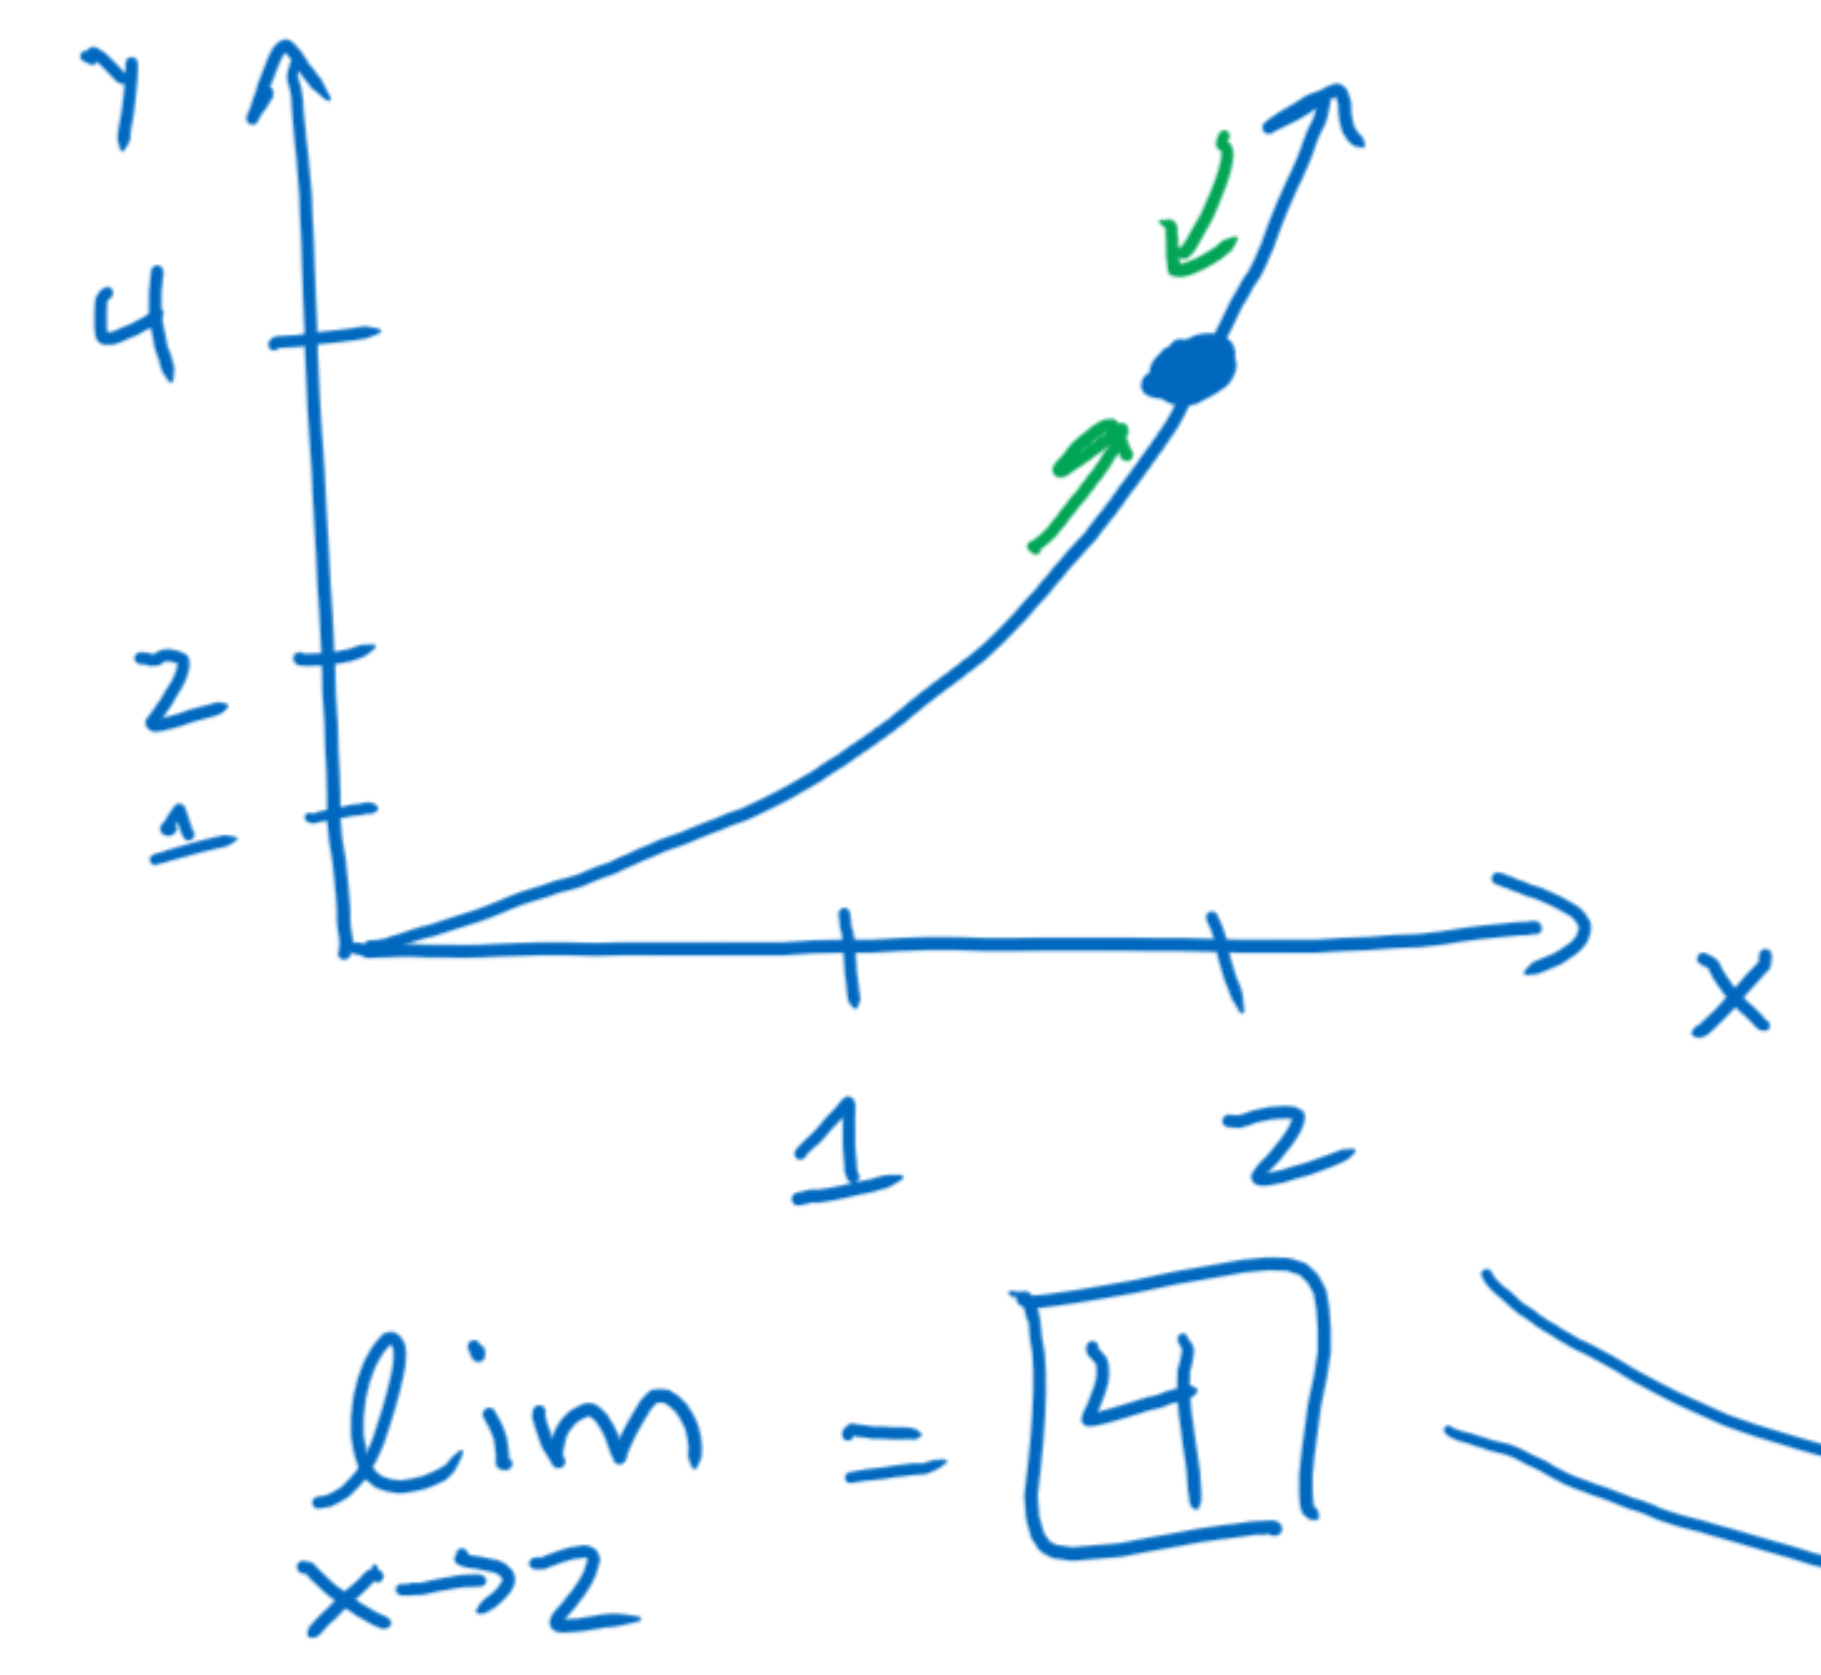
\includegraphics[width = 10cm]{images/1.2_Image.PNG}
	\end{center}
\end{figure*}

\begin{itemize}
	\item In the example above, the limit is 4 because the function output as you approach 2 from the left is equal to the function output as you approach 2 from the right
	\item Because there can be possible issues with scale, graphical representations of limits can possibly be inaccurate and can miss important behaviors of functions if you're too far zoomed out
	\item A limit can fail to exist at particular values of $x$ if LHL $\ne$ RHL, the function oscillates near $x$, or if the function is unbounded
\end{itemize}
\newpage

\section{Estimating Limit Values From Tables}

\begin{itemize}
	\item Numerical information from tables can be used to estimate Limits
\end{itemize}

\begin{figure*}
	\begin{center}
		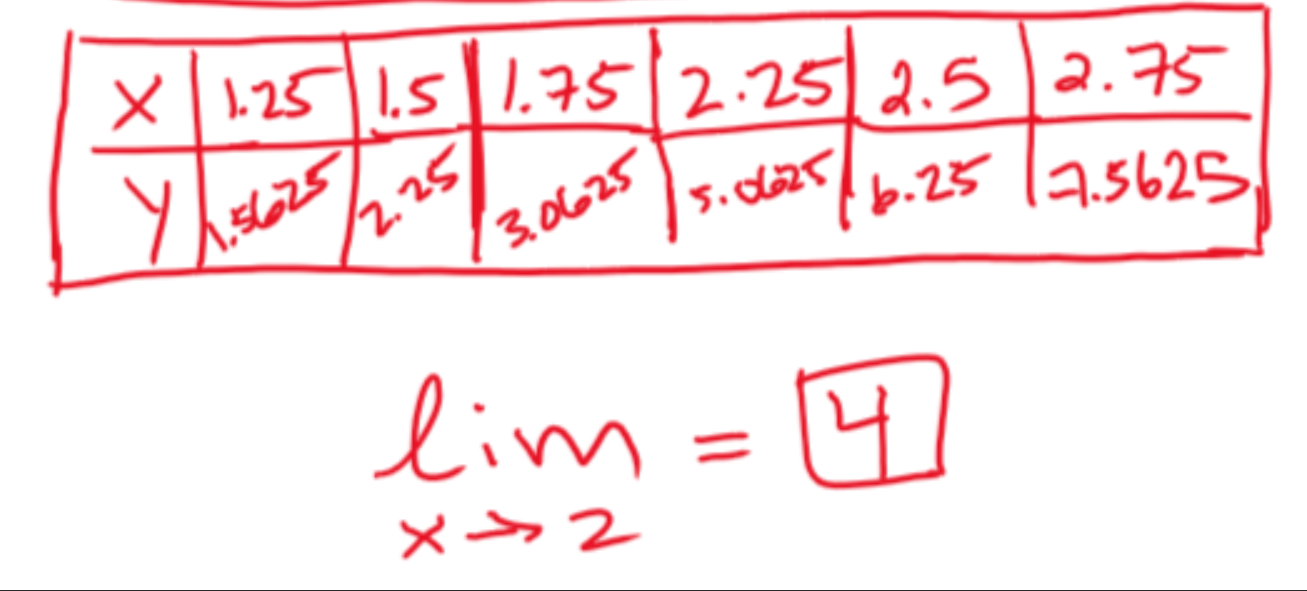
\includegraphics[width=10cm]{images/1.4_Image.PNG}
	\end{center}
\end{figure*}

\begin{itemize}
	\item As seen in the table, the output values for 1.75 and below all seem to be getting closer to 4 while $x$ gets larger,
	while the output values for 2.25 and greater all have values approaching 4 as $x$ gets smaller. Since the LHL is equal to the RHL, we can conclude that the limit as $x$ approaches 2 is indeed 4 
\end{itemize}

\section{Determining Limits Using Algebraic Properties of Limits}
% Maybe come back and make a prettier table in the future, but for now just keep the image

\begin{figure*}
	\begin{center}
		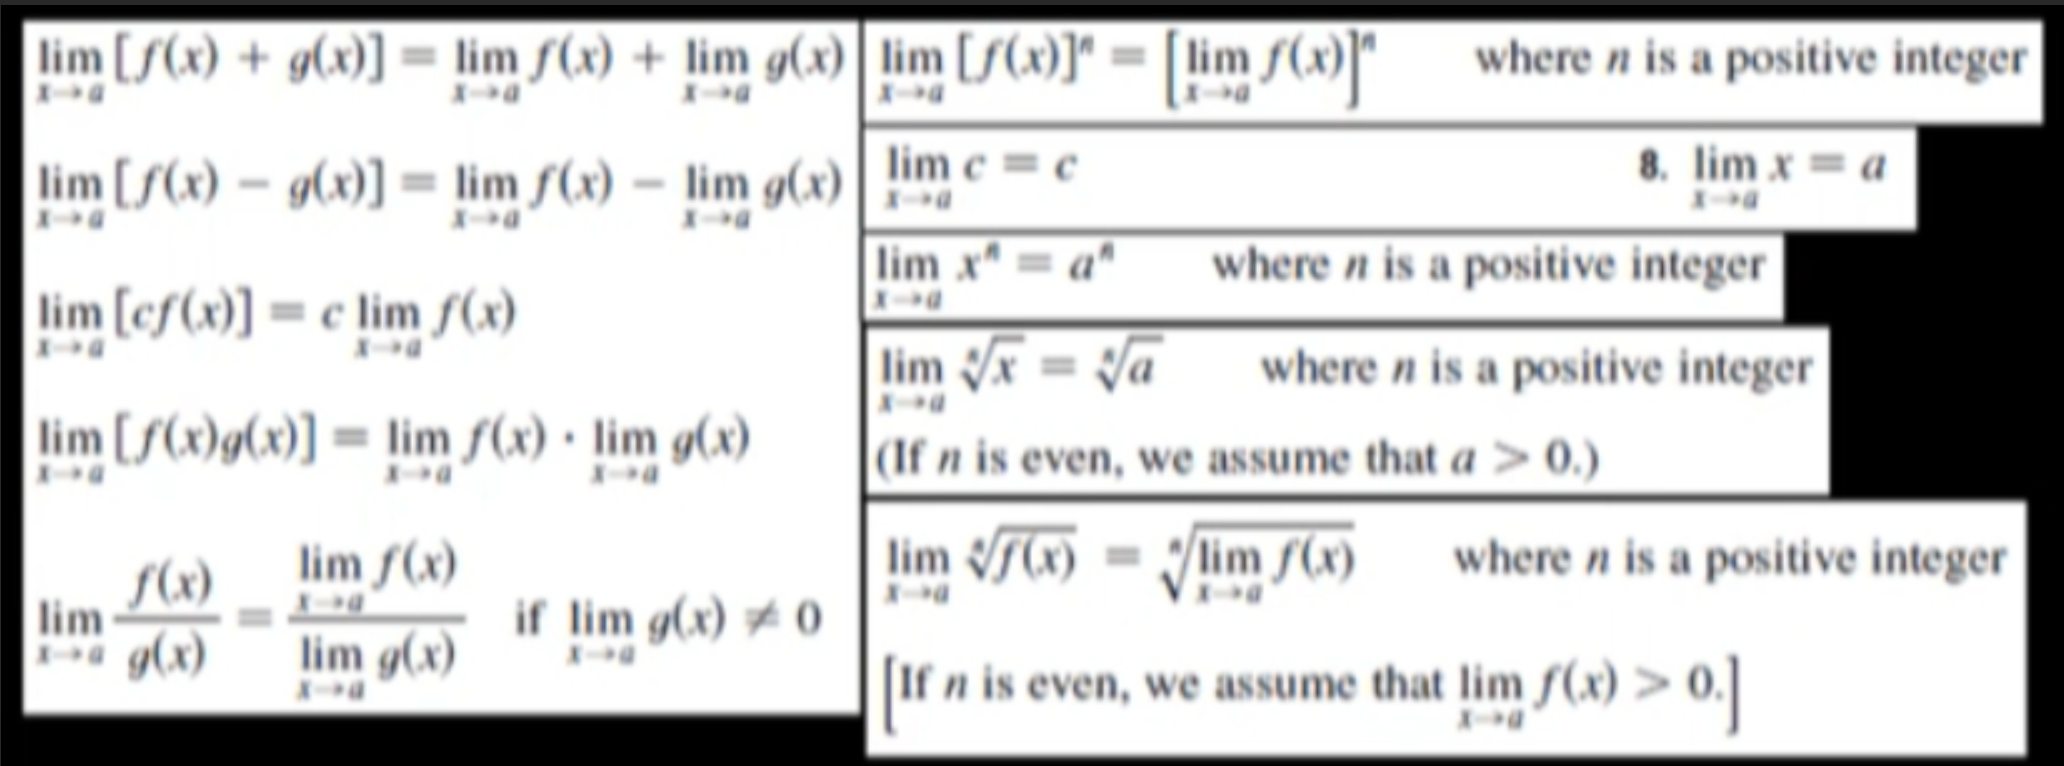
\includegraphics[width=10cm]{images/1.5_Image.PNG}
	\end{center}
\end{figure*}

\begin{itemize}
	\item To evaluate a limit, simply substitute the desired value that you wish to find the limit at
\end{itemize}

\end{document}
.